\documentclass[twoside]{book}

% Packages required by doxygen
\usepackage{calc}
\usepackage{doxygen}
\usepackage{graphicx}
\usepackage[utf8]{inputenc}
\usepackage{makeidx}
\usepackage{multicol}
\usepackage{multirow}
\usepackage{textcomp}
\usepackage[table]{xcolor}

% Font selection
\usepackage[T1]{fontenc}
\usepackage{mathptmx}
\usepackage[scaled=.90]{helvet}
\usepackage{courier}
\usepackage{amssymb}
\usepackage{sectsty}
\renewcommand{\familydefault}{\sfdefault}
\allsectionsfont{%
  \fontseries{bc}\selectfont%
  \color{darkgray}%
}
\renewcommand{\DoxyLabelFont}{%
  \fontseries{bc}\selectfont%
  \color{darkgray}%
}

% Page & text layout
\usepackage{geometry}
\geometry{%
  a4paper,%
  top=2.5cm,%
  bottom=2.5cm,%
  left=2.5cm,%
  right=2.5cm%
}
\tolerance=750
\hfuzz=15pt
\hbadness=750
\setlength{\emergencystretch}{15pt}
\setlength{\parindent}{0cm}
\setlength{\parskip}{0.2cm}
\makeatletter
\renewcommand{\paragraph}{%
  \@startsection{paragraph}{4}{0ex}{-1.0ex}{1.0ex}{%
    \normalfont\normalsize\bfseries\SS@parafont%
  }%
}
\renewcommand{\subparagraph}{%
  \@startsection{subparagraph}{5}{0ex}{-1.0ex}{1.0ex}{%
    \normalfont\normalsize\bfseries\SS@subparafont%
  }%
}
\makeatother

% Headers & footers
\usepackage{fancyhdr}
\pagestyle{fancyplain}
\fancyhead[LE]{\fancyplain{}{\bfseries\thepage}}
\fancyhead[CE]{\fancyplain{}{}}
\fancyhead[RE]{\fancyplain{}{\bfseries\leftmark}}
\fancyhead[LO]{\fancyplain{}{\bfseries\rightmark}}
\fancyhead[CO]{\fancyplain{}{}}
\fancyhead[RO]{\fancyplain{}{\bfseries\thepage}}
\fancyfoot[LE]{\fancyplain{}{}}
\fancyfoot[CE]{\fancyplain{}{}}
\fancyfoot[RE]{\fancyplain{}{\bfseries\scriptsize Generated on Tue Oct 8 2013 22:49:19 for Andengine-anchor-center by Doxygen }}
\fancyfoot[LO]{\fancyplain{}{\bfseries\scriptsize Generated on Tue Oct 8 2013 22:49:19 for Andengine-anchor-center by Doxygen }}
\fancyfoot[CO]{\fancyplain{}{}}
\fancyfoot[RO]{\fancyplain{}{}}
\renewcommand{\footrulewidth}{0.4pt}
\renewcommand{\chaptermark}[1]{%
  \markboth{#1}{}%
}
\renewcommand{\sectionmark}[1]{%
  \markright{\thesection\ #1}%
}

% Indices & bibliography
\usepackage{natbib}
\usepackage[titles]{tocloft}
\setcounter{tocdepth}{3}
\setcounter{secnumdepth}{5}
\makeindex

% Hyperlinks (required, but should be loaded last)
\usepackage{ifpdf}
\ifpdf
  \usepackage[pdftex,pagebackref=true]{hyperref}
\else
  \usepackage[ps2pdf,pagebackref=true]{hyperref}
\fi
\hypersetup{%
  colorlinks=true,%
  linkcolor=blue,%
  citecolor=blue,%
  unicode%
}

% Custom commands
\newcommand{\clearemptydoublepage}{%
  \newpage{\pagestyle{empty}\cleardoublepage}%
}


%===== C O N T E N T S =====

\begin{document}

% Titlepage & ToC
\hypersetup{pageanchor=false}
\pagenumbering{roman}
\begin{titlepage}
\vspace*{7cm}
\begin{center}%
{\Large Andengine-\/anchor-\/center }\\
\vspace*{1cm}
{\large Generated by Doxygen 1.8.4}\\
\vspace*{0.5cm}
{\small Tue Oct 8 2013 22:49:19}\\
\end{center}
\end{titlepage}
\clearemptydoublepage
\tableofcontents
\clearemptydoublepage
\pagenumbering{arabic}
\hypersetup{pageanchor=true}

%--- Begin generated contents ---
\chapter{Namespace Index}
\section{Packages}
Here are the packages with brief descriptions (if available)\-:\begin{DoxyCompactList}
\item\contentsline{section}{\hyperlink{namespacecom}{com} }{\pageref{namespacecom}}{}
\item\contentsline{section}{\hyperlink{namespacecom_1_1tuukka}{com.\-tuukka} }{\pageref{namespacecom_1_1tuukka}}{}
\item\contentsline{section}{\hyperlink{namespacecom_1_1tuukka_1_1fromscratch}{com.\-tuukka.\-fromscratch} }{\pageref{namespacecom_1_1tuukka_1_1fromscratch}}{}
\end{DoxyCompactList}

\chapter{Hierarchical Index}
\section{Class Hierarchy}
This inheritance list is sorted roughly, but not completely, alphabetically\-:\begin{DoxyCompactList}
\item \contentsline{section}{com.\-tuukka.\-fromscratch.\-Build\-Config}{\pageref{classcom_1_1tuukka_1_1fromscratch_1_1BuildConfig}}{}
\item \contentsline{section}{com.\-tuukka.\-fromscratch.\-Game\-Manager}{\pageref{classcom_1_1tuukka_1_1fromscratch_1_1GameManager}}{}
\item \contentsline{section}{com.\-tuukka.\-fromscratch.\-R}{\pageref{classcom_1_1tuukka_1_1fromscratch_1_1R}}{}
\item Simple\-Base\-Game\-Activity\begin{DoxyCompactList}
\item \contentsline{section}{com.\-tuukka.\-fromscratch.\-Main}{\pageref{classcom_1_1tuukka_1_1fromscratch_1_1Main}}{}
\end{DoxyCompactList}
\end{DoxyCompactList}

\chapter{Class Index}
\section{Class List}
Here are the classes, structs, unions and interfaces with brief descriptions\-:\begin{DoxyCompactList}
\item\contentsline{section}{\hyperlink{classcom_1_1tuukka_1_1fromscratch_1_1BuildConfig}{com.\-tuukka.\-fromscratch.\-Build\-Config} }{\pageref{classcom_1_1tuukka_1_1fromscratch_1_1BuildConfig}}{}
\item\contentsline{section}{\hyperlink{classcom_1_1tuukka_1_1fromscratch_1_1GameManager}{com.\-tuukka.\-fromscratch.\-Game\-Manager} }{\pageref{classcom_1_1tuukka_1_1fromscratch_1_1GameManager}}{}
\item\contentsline{section}{\hyperlink{classcom_1_1tuukka_1_1fromscratch_1_1Main}{com.\-tuukka.\-fromscratch.\-Main} }{\pageref{classcom_1_1tuukka_1_1fromscratch_1_1Main}}{}
\item\contentsline{section}{\hyperlink{classcom_1_1tuukka_1_1fromscratch_1_1R}{com.\-tuukka.\-fromscratch.\-R} }{\pageref{classcom_1_1tuukka_1_1fromscratch_1_1R}}{}
\end{DoxyCompactList}

\chapter{File Index}
\section{File List}
Here is a list of all files with brief descriptions\-:\begin{DoxyCompactList}
\item\contentsline{section}{gen/com/tuukka/fromscratch/\hyperlink{BuildConfig_8java}{Build\-Config.\-java} }{\pageref{BuildConfig_8java}}{}
\item\contentsline{section}{gen/com/tuukka/fromscratch/\hyperlink{R_8java}{R.\-java} }{\pageref{R_8java}}{}
\item\contentsline{section}{src/com/tuukka/fromscratch/\hyperlink{GameManager_8java}{Game\-Manager.\-java} }{\pageref{GameManager_8java}}{}
\item\contentsline{section}{src/com/tuukka/fromscratch/\hyperlink{Main_8java}{Main.\-java} }{\pageref{Main_8java}}{}
\end{DoxyCompactList}

\chapter{Namespace Documentation}
\hypertarget{namespacecom}{\section{Package com}
\label{namespacecom}\index{com@{com}}
}
\subsection*{Packages}
\begin{DoxyCompactItemize}
\item 
package \hyperlink{namespacecom_1_1tuukka}{tuukka}
\end{DoxyCompactItemize}

\hypertarget{namespacecom_1_1tuukka}{\section{Package com.\-tuukka}
\label{namespacecom_1_1tuukka}\index{com.\-tuukka@{com.\-tuukka}}
}
\subsection*{Packages}
\begin{DoxyCompactItemize}
\item 
package \hyperlink{namespacecom_1_1tuukka_1_1fromscratch}{fromscratch}
\end{DoxyCompactItemize}

\hypertarget{namespacecom_1_1tuukka_1_1fromscratch}{\section{Package com.\-tuukka.\-fromscratch}
\label{namespacecom_1_1tuukka_1_1fromscratch}\index{com.\-tuukka.\-fromscratch@{com.\-tuukka.\-fromscratch}}
}
\subsection*{Classes}
\begin{DoxyCompactItemize}
\item 
class \hyperlink{classcom_1_1tuukka_1_1fromscratch_1_1BuildConfig}{Build\-Config}
\item 
class \hyperlink{classcom_1_1tuukka_1_1fromscratch_1_1R}{R}
\item 
class \hyperlink{classcom_1_1tuukka_1_1fromscratch_1_1GameManager}{Game\-Manager}
\item 
class \hyperlink{classcom_1_1tuukka_1_1fromscratch_1_1Main}{Main}
\end{DoxyCompactItemize}


\subsection{Detailed Description}
Automatically generated file. D\-O N\-O\-T M\-O\-D\-I\-F\-Y 
\chapter{Class Documentation}
\hypertarget{classcom_1_1tuukka_1_1fromscratch_1_1BuildConfig}{\section{com.\-tuukka.\-fromscratch.\-Build\-Config Class Reference}
\label{classcom_1_1tuukka_1_1fromscratch_1_1BuildConfig}\index{com.\-tuukka.\-fromscratch.\-Build\-Config@{com.\-tuukka.\-fromscratch.\-Build\-Config}}
}


Collaboration diagram for com.\-tuukka.\-fromscratch.\-Build\-Config\-:
\nopagebreak
\begin{figure}[H]
\begin{center}
\leavevmode
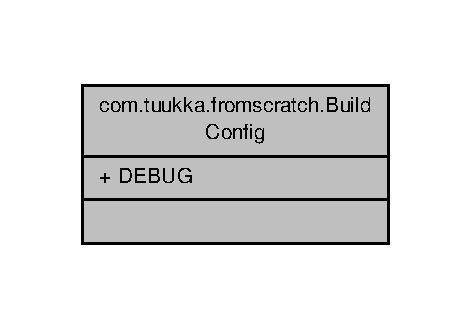
\includegraphics[width=226pt]{classcom_1_1tuukka_1_1fromscratch_1_1BuildConfig__coll__graph}
\end{center}
\end{figure}
\subsection*{Static Public Attributes}
\begin{DoxyCompactItemize}
\item 
static final boolean \hyperlink{classcom_1_1tuukka_1_1fromscratch_1_1BuildConfig_a0ee977c60db1caa42d16f94dd93d52e3}{D\-E\-B\-U\-G} = true
\end{DoxyCompactItemize}


\subsection{Member Data Documentation}
\hypertarget{classcom_1_1tuukka_1_1fromscratch_1_1BuildConfig_a0ee977c60db1caa42d16f94dd93d52e3}{\index{com\-::tuukka\-::fromscratch\-::\-Build\-Config@{com\-::tuukka\-::fromscratch\-::\-Build\-Config}!D\-E\-B\-U\-G@{D\-E\-B\-U\-G}}
\index{D\-E\-B\-U\-G@{D\-E\-B\-U\-G}!com::tuukka::fromscratch::BuildConfig@{com\-::tuukka\-::fromscratch\-::\-Build\-Config}}
\subsubsection[{D\-E\-B\-U\-G}]{\setlength{\rightskip}{0pt plus 5cm}final boolean com.\-tuukka.\-fromscratch.\-Build\-Config.\-D\-E\-B\-U\-G = true\hspace{0.3cm}{\ttfamily [static]}}}\label{classcom_1_1tuukka_1_1fromscratch_1_1BuildConfig_a0ee977c60db1caa42d16f94dd93d52e3}


The documentation for this class was generated from the following file\-:\begin{DoxyCompactItemize}
\item 
gen/com/tuukka/fromscratch/\hyperlink{BuildConfig_8java}{Build\-Config.\-java}\end{DoxyCompactItemize}

\hypertarget{classcom_1_1tuukka_1_1fromscratch_1_1GameManager}{\section{com.\-tuukka.\-fromscratch.\-Game\-Manager Class Reference}
\label{classcom_1_1tuukka_1_1fromscratch_1_1GameManager}\index{com.\-tuukka.\-fromscratch.\-Game\-Manager@{com.\-tuukka.\-fromscratch.\-Game\-Manager}}
}


Collaboration diagram for com.\-tuukka.\-fromscratch.\-Game\-Manager\-:
\nopagebreak
\begin{figure}[H]
\begin{center}
\leavevmode
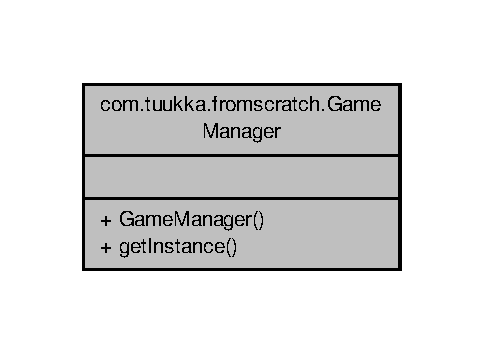
\includegraphics[width=232pt]{classcom_1_1tuukka_1_1fromscratch_1_1GameManager__coll__graph}
\end{center}
\end{figure}
\subsection*{Public Member Functions}
\begin{DoxyCompactItemize}
\item 
\hyperlink{classcom_1_1tuukka_1_1fromscratch_1_1GameManager_a1983c0111eadbad425f1f7f6d45d1e45}{Game\-Manager} ()
\end{DoxyCompactItemize}
\subsection*{Static Public Member Functions}
\begin{DoxyCompactItemize}
\item 
static \hyperlink{classcom_1_1tuukka_1_1fromscratch_1_1GameManager}{Game\-Manager} \hyperlink{classcom_1_1tuukka_1_1fromscratch_1_1GameManager_ac41cf4fead39f5943ff0ed37b025085c}{get\-Instance} ()
\end{DoxyCompactItemize}


\subsection{Constructor \& Destructor Documentation}
\hypertarget{classcom_1_1tuukka_1_1fromscratch_1_1GameManager_a1983c0111eadbad425f1f7f6d45d1e45}{\index{com\-::tuukka\-::fromscratch\-::\-Game\-Manager@{com\-::tuukka\-::fromscratch\-::\-Game\-Manager}!Game\-Manager@{Game\-Manager}}
\index{Game\-Manager@{Game\-Manager}!com::tuukka::fromscratch::GameManager@{com\-::tuukka\-::fromscratch\-::\-Game\-Manager}}
\subsubsection[{Game\-Manager}]{\setlength{\rightskip}{0pt plus 5cm}com.\-tuukka.\-fromscratch.\-Game\-Manager.\-Game\-Manager (
\begin{DoxyParamCaption}
{}
\end{DoxyParamCaption}
)}}\label{classcom_1_1tuukka_1_1fromscratch_1_1GameManager_a1983c0111eadbad425f1f7f6d45d1e45}


\subsection{Member Function Documentation}
\hypertarget{classcom_1_1tuukka_1_1fromscratch_1_1GameManager_ac41cf4fead39f5943ff0ed37b025085c}{\index{com\-::tuukka\-::fromscratch\-::\-Game\-Manager@{com\-::tuukka\-::fromscratch\-::\-Game\-Manager}!get\-Instance@{get\-Instance}}
\index{get\-Instance@{get\-Instance}!com::tuukka::fromscratch::GameManager@{com\-::tuukka\-::fromscratch\-::\-Game\-Manager}}
\subsubsection[{get\-Instance}]{\setlength{\rightskip}{0pt plus 5cm}static {\bf Game\-Manager} com.\-tuukka.\-fromscratch.\-Game\-Manager.\-get\-Instance (
\begin{DoxyParamCaption}
{}
\end{DoxyParamCaption}
)\hspace{0.3cm}{\ttfamily [static]}}}\label{classcom_1_1tuukka_1_1fromscratch_1_1GameManager_ac41cf4fead39f5943ff0ed37b025085c}


The documentation for this class was generated from the following file\-:\begin{DoxyCompactItemize}
\item 
src/com/tuukka/fromscratch/\hyperlink{GameManager_8java}{Game\-Manager.\-java}\end{DoxyCompactItemize}

\hypertarget{classcom_1_1tuukka_1_1fromscratch_1_1Main}{\section{com.\-tuukka.\-fromscratch.\-Main Class Reference}
\label{classcom_1_1tuukka_1_1fromscratch_1_1Main}\index{com.\-tuukka.\-fromscratch.\-Main@{com.\-tuukka.\-fromscratch.\-Main}}
}


Inheritance diagram for com.\-tuukka.\-fromscratch.\-Main\-:
\nopagebreak
\begin{figure}[H]
\begin{center}
\leavevmode
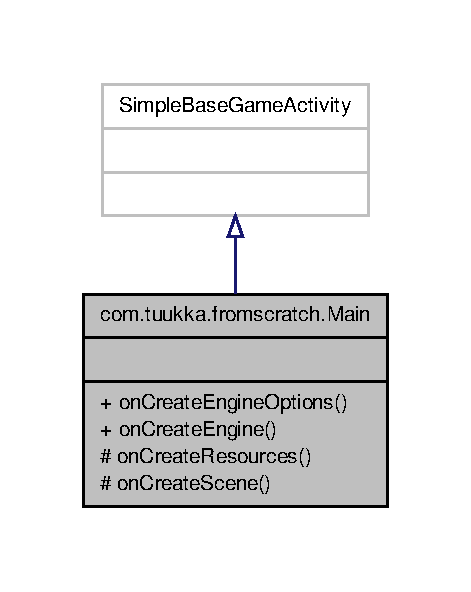
\includegraphics[width=226pt]{classcom_1_1tuukka_1_1fromscratch_1_1Main__inherit__graph}
\end{center}
\end{figure}


Collaboration diagram for com.\-tuukka.\-fromscratch.\-Main\-:
\nopagebreak
\begin{figure}[H]
\begin{center}
\leavevmode
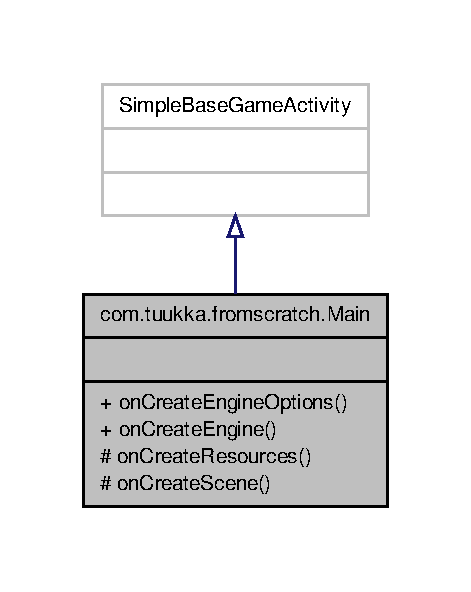
\includegraphics[width=226pt]{classcom_1_1tuukka_1_1fromscratch_1_1Main__coll__graph}
\end{center}
\end{figure}
\subsection*{Public Member Functions}
\begin{DoxyCompactItemize}
\item 
Engine\-Options \hyperlink{classcom_1_1tuukka_1_1fromscratch_1_1Main_ab6d1a0dfa642b3a770bba2a0ab398e8f}{on\-Create\-Engine\-Options} ()
\item 
Engine \hyperlink{classcom_1_1tuukka_1_1fromscratch_1_1Main_a657a41f97bb56332933b35a67fcfe879}{on\-Create\-Engine} (Engine\-Options p\-Engine\-Options)
\end{DoxyCompactItemize}
\subsection*{Protected Member Functions}
\begin{DoxyCompactItemize}
\item 
void \hyperlink{classcom_1_1tuukka_1_1fromscratch_1_1Main_ab018eb79e77d9dadef45f947a14d5625}{on\-Create\-Resources} ()  throws I\-O\-Exception 
\item 
Scene \hyperlink{classcom_1_1tuukka_1_1fromscratch_1_1Main_a3296880ced15a386337e05b3e7e00d5a}{on\-Create\-Scene} ()
\end{DoxyCompactItemize}


\subsection{Member Function Documentation}
\hypertarget{classcom_1_1tuukka_1_1fromscratch_1_1Main_a657a41f97bb56332933b35a67fcfe879}{\index{com\-::tuukka\-::fromscratch\-::\-Main@{com\-::tuukka\-::fromscratch\-::\-Main}!on\-Create\-Engine@{on\-Create\-Engine}}
\index{on\-Create\-Engine@{on\-Create\-Engine}!com::tuukka::fromscratch::Main@{com\-::tuukka\-::fromscratch\-::\-Main}}
\subsubsection[{on\-Create\-Engine}]{\setlength{\rightskip}{0pt plus 5cm}Engine com.\-tuukka.\-fromscratch.\-Main.\-on\-Create\-Engine (
\begin{DoxyParamCaption}
\item[{Engine\-Options}]{p\-Engine\-Options}
\end{DoxyParamCaption}
)}}\label{classcom_1_1tuukka_1_1fromscratch_1_1Main_a657a41f97bb56332933b35a67fcfe879}
\hypertarget{classcom_1_1tuukka_1_1fromscratch_1_1Main_ab6d1a0dfa642b3a770bba2a0ab398e8f}{\index{com\-::tuukka\-::fromscratch\-::\-Main@{com\-::tuukka\-::fromscratch\-::\-Main}!on\-Create\-Engine\-Options@{on\-Create\-Engine\-Options}}
\index{on\-Create\-Engine\-Options@{on\-Create\-Engine\-Options}!com::tuukka::fromscratch::Main@{com\-::tuukka\-::fromscratch\-::\-Main}}
\subsubsection[{on\-Create\-Engine\-Options}]{\setlength{\rightskip}{0pt plus 5cm}Engine\-Options com.\-tuukka.\-fromscratch.\-Main.\-on\-Create\-Engine\-Options (
\begin{DoxyParamCaption}
{}
\end{DoxyParamCaption}
)}}\label{classcom_1_1tuukka_1_1fromscratch_1_1Main_ab6d1a0dfa642b3a770bba2a0ab398e8f}
\hypertarget{classcom_1_1tuukka_1_1fromscratch_1_1Main_ab018eb79e77d9dadef45f947a14d5625}{\index{com\-::tuukka\-::fromscratch\-::\-Main@{com\-::tuukka\-::fromscratch\-::\-Main}!on\-Create\-Resources@{on\-Create\-Resources}}
\index{on\-Create\-Resources@{on\-Create\-Resources}!com::tuukka::fromscratch::Main@{com\-::tuukka\-::fromscratch\-::\-Main}}
\subsubsection[{on\-Create\-Resources}]{\setlength{\rightskip}{0pt plus 5cm}void com.\-tuukka.\-fromscratch.\-Main.\-on\-Create\-Resources (
\begin{DoxyParamCaption}
{}
\end{DoxyParamCaption}
) throws I\-O\-Exception\hspace{0.3cm}{\ttfamily [protected]}}}\label{classcom_1_1tuukka_1_1fromscratch_1_1Main_ab018eb79e77d9dadef45f947a14d5625}
\hypertarget{classcom_1_1tuukka_1_1fromscratch_1_1Main_a3296880ced15a386337e05b3e7e00d5a}{\index{com\-::tuukka\-::fromscratch\-::\-Main@{com\-::tuukka\-::fromscratch\-::\-Main}!on\-Create\-Scene@{on\-Create\-Scene}}
\index{on\-Create\-Scene@{on\-Create\-Scene}!com::tuukka::fromscratch::Main@{com\-::tuukka\-::fromscratch\-::\-Main}}
\subsubsection[{on\-Create\-Scene}]{\setlength{\rightskip}{0pt plus 5cm}Scene com.\-tuukka.\-fromscratch.\-Main.\-on\-Create\-Scene (
\begin{DoxyParamCaption}
{}
\end{DoxyParamCaption}
)\hspace{0.3cm}{\ttfamily [protected]}}}\label{classcom_1_1tuukka_1_1fromscratch_1_1Main_a3296880ced15a386337e05b3e7e00d5a}


The documentation for this class was generated from the following file\-:\begin{DoxyCompactItemize}
\item 
src/com/tuukka/fromscratch/\hyperlink{Main_8java}{Main.\-java}\end{DoxyCompactItemize}

\hypertarget{classcom_1_1tuukka_1_1fromscratch_1_1R}{\section{com.\-tuukka.\-fromscratch.\-R Class Reference}
\label{classcom_1_1tuukka_1_1fromscratch_1_1R}\index{com.\-tuukka.\-fromscratch.\-R@{com.\-tuukka.\-fromscratch.\-R}}
}


Collaboration diagram for com.\-tuukka.\-fromscratch.\-R\-:
\nopagebreak
\begin{figure}[H]
\begin{center}
\leavevmode
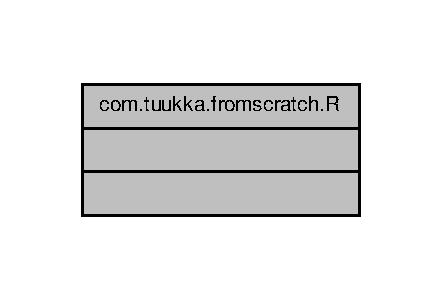
\includegraphics[width=212pt]{classcom_1_1tuukka_1_1fromscratch_1_1R__coll__graph}
\end{center}
\end{figure}
\subsection*{Classes}
\begin{DoxyCompactItemize}
\item 
class {\bfseries attr}
\item 
class {\bfseries drawable}
\item 
class {\bfseries string}
\item 
class {\bfseries style}
\end{DoxyCompactItemize}


The documentation for this class was generated from the following file\-:\begin{DoxyCompactItemize}
\item 
gen/com/tuukka/fromscratch/\hyperlink{R_8java}{R.\-java}\end{DoxyCompactItemize}

\chapter{File Documentation}
\hypertarget{BuildConfig_8java}{\section{gen/com/tuukka/fromscratch/\-Build\-Config.java File Reference}
\label{BuildConfig_8java}\index{gen/com/tuukka/fromscratch/\-Build\-Config.\-java@{gen/com/tuukka/fromscratch/\-Build\-Config.\-java}}
}
\subsection*{Classes}
\begin{DoxyCompactItemize}
\item 
class \hyperlink{classcom_1_1tuukka_1_1fromscratch_1_1BuildConfig}{com.\-tuukka.\-fromscratch.\-Build\-Config}
\end{DoxyCompactItemize}
\subsection*{Packages}
\begin{DoxyCompactItemize}
\item 
package \hyperlink{namespacecom_1_1tuukka_1_1fromscratch}{com.\-tuukka.\-fromscratch}
\end{DoxyCompactItemize}
\subsection*{Constant Groups}
\begin{DoxyCompactItemize}
\item 
package \hyperlink{namespacecom_1_1tuukka_1_1fromscratch}{com.\-tuukka.\-fromscratch}
\end{DoxyCompactItemize}

\hypertarget{R_8java}{\section{gen/com/tuukka/fromscratch/\-R.java File Reference}
\label{R_8java}\index{gen/com/tuukka/fromscratch/\-R.\-java@{gen/com/tuukka/fromscratch/\-R.\-java}}
}
\subsection*{Classes}
\begin{DoxyCompactItemize}
\item 
class \hyperlink{classcom_1_1tuukka_1_1fromscratch_1_1R}{com.\-tuukka.\-fromscratch.\-R}
\item 
class {\bfseries com.\-tuukka.\-fromscratch.\-R.\-attr}
\item 
class {\bfseries com.\-tuukka.\-fromscratch.\-R.\-drawable}
\item 
class {\bfseries com.\-tuukka.\-fromscratch.\-R.\-string}
\item 
class {\bfseries com.\-tuukka.\-fromscratch.\-R.\-style}
\end{DoxyCompactItemize}
\subsection*{Packages}
\begin{DoxyCompactItemize}
\item 
package \hyperlink{namespacecom_1_1tuukka_1_1fromscratch}{com.\-tuukka.\-fromscratch}
\end{DoxyCompactItemize}
\subsection*{Constant Groups}
\begin{DoxyCompactItemize}
\item 
package \hyperlink{namespacecom_1_1tuukka_1_1fromscratch}{com.\-tuukka.\-fromscratch}
\end{DoxyCompactItemize}

\hypertarget{GameManager_8java}{\section{src/com/tuukka/fromscratch/\-Game\-Manager.java File Reference}
\label{GameManager_8java}\index{src/com/tuukka/fromscratch/\-Game\-Manager.\-java@{src/com/tuukka/fromscratch/\-Game\-Manager.\-java}}
}
\subsection*{Classes}
\begin{DoxyCompactItemize}
\item 
class \hyperlink{classcom_1_1tuukka_1_1fromscratch_1_1GameManager}{com.\-tuukka.\-fromscratch.\-Game\-Manager}
\end{DoxyCompactItemize}
\subsection*{Packages}
\begin{DoxyCompactItemize}
\item 
package \hyperlink{namespacecom_1_1tuukka_1_1fromscratch}{com.\-tuukka.\-fromscratch}
\end{DoxyCompactItemize}
\subsection*{Constant Groups}
\begin{DoxyCompactItemize}
\item 
package \hyperlink{namespacecom_1_1tuukka_1_1fromscratch}{com.\-tuukka.\-fromscratch}
\end{DoxyCompactItemize}

\hypertarget{Main_8java}{\section{src/com/tuukka/fromscratch/\-Main.java File Reference}
\label{Main_8java}\index{src/com/tuukka/fromscratch/\-Main.\-java@{src/com/tuukka/fromscratch/\-Main.\-java}}
}
\subsection*{Classes}
\begin{DoxyCompactItemize}
\item 
class \hyperlink{classcom_1_1tuukka_1_1fromscratch_1_1Main}{com.\-tuukka.\-fromscratch.\-Main}
\end{DoxyCompactItemize}
\subsection*{Packages}
\begin{DoxyCompactItemize}
\item 
package \hyperlink{namespacecom_1_1tuukka_1_1fromscratch}{com.\-tuukka.\-fromscratch}
\end{DoxyCompactItemize}
\subsection*{Constant Groups}
\begin{DoxyCompactItemize}
\item 
package \hyperlink{namespacecom_1_1tuukka_1_1fromscratch}{com.\-tuukka.\-fromscratch}
\end{DoxyCompactItemize}

%--- End generated contents ---

% Index
\newpage
\phantomsection
\addcontentsline{toc}{part}{Index}
\printindex

\end{document}
